\chapter{Revue de littérature}
\label{ch:litterature}

\section{Historique et concepts de la RA}
\label{sec:litterature_ar_presentation}

\cite{Sutherland1968} conçoit le premier visiocasque de RA \figrefp{Sutherland1968} : ce prototype permet déjà de visualiser du contenu 3D affiché dans l'espace réel de l'utilisateur, donnant l'illusion que le contenu virtuel fait réellement partie de la pièce. Par la suite, la recherche académique en RA se développe lentement : les applications développées sont surtout à visées militaires et gouvernementales \citep{VanKrevelen2010}. Il faut alors attendre les années 1990, avec la miniaturisation des PCs, pour que le domaine de recherche s'établisse enfin. Plusieurs conférences dédiées à la RA sont notamment créées, fusionnées aujourd'hui sous le nom d'International Symposium on Mixed and Augmented Reality (ISMAR), une conférence d'importance pour la recherche et l'industrie en RA \citep{Azuma2001}.

\figureETS[0.6]{Sutherland1968}{
  Photos du visiocasque de RA de Sutherland.\\
  Tiré de \cite{Sutherland1968}.
}

\cite{Milgram1994} donne un premier cadre théorique au domaine, en proposant une échelle ordonnée nommée \texten{Reality-Virtuality Continuum} \figrefp{Milgram1994}. \citeauthor{Milgram1994} y oppose deux extrêmes : les environnements réels et les environnements virtuels. Les IHMs graphiques, en deux dimensions (2D), sur ordinateurs et téléphones font partie de la première catégorie, tandis que les visiocasques de RV, qui immergent totalement leurs utilisateurs dans un monde virtuel en 3D, de la seconde. Entre ces deux extrêmes, les environnements de Réalité Mixte (RM), comme la RA, vont mélanger éléments réels et virtuels. La force de cette représentation est qu'il n'existe pas de catégories séparées entre réel, RA et RV mais que la RA peut se trouver d'un extrême à un autre le long de cette échelle.

Le second enseignement de l'échelle de \citeauthor{Milgram1994} est que RA et RV sont techniquement très proches : les dispositifs de localisation, d'affichage et de génération de contenu sont les mêmes \citep{Billinghurst2015}. Cependant, ces deux technologies n'ont pas les mêmes attentes. En effet, pour que l'immersion en RV fonctionne, il est nécessaire d'avoir un large champ de vision (\texten{field of view} ou FoV en anglais) ; par exemple, le champ de vision du visiocasque de RV HTC Vive est de \SI{100x113}{\degree} (horizontalement $\times$ verticalement) pour les deux yeux \citep{Kreylos2016}, ce qui est assez proche du champ de vision humain de \SI{200x120}{\degree} pour les deux yeux \citep{Cockburn2008}. La RA va en revanche demander tout d'abord une très grande précision et rapidité dans la localisation de l'utilisateur et des objets à augmenter pour donner le sentiment de « présence » du virtuel dans l'environnement réel.

\figureLayoutETS{Milgram1994}{%
  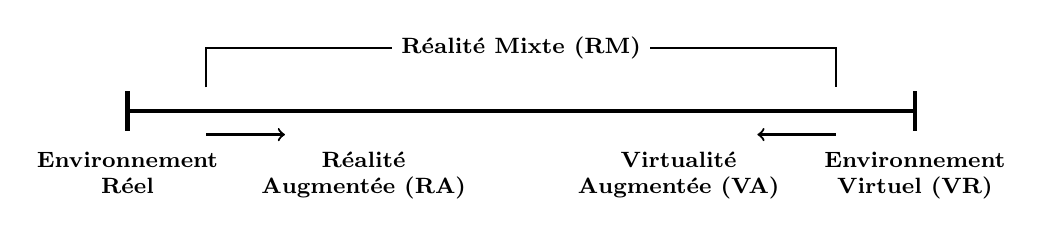
\begin{tikzpicture}[font=\footnotesize\bfseries]
    \tikzstyle{label}=[below, align=center, text depth=.25ex]
    
    \draw[ultra thick] (0,0) -- (10,0);
    \draw[ultra thick] (0,-0.25) -- (0,0.25);
    \draw[ultra thick] (10,-0.25) -- (10,0.25);

    \draw[thick, ->] (1,-0.3) -- (2,-0.3);
    \draw[thick, <-] (8,-0.3) -- (9,-0.3);

    \draw (0,-0.4) node[label] {Environnement\\Réel};
    \draw (3,-0.4) node[label] {Réalité\\Augmentée (RA)};
    \draw (7,-0.4) node[label] {Virtualité\\Augmentée (VA)};
    \draw (10,-0.4) node[label] {Environnement\\Virtuel (VR)};

    \draw[thick] (1,0.3) -- (1,0.8) -- (9,0.8) -- (9,0.3);

    \draw (5,0.8) node[fill=white] {Réalité Mixte (RM)};
  \end{tikzpicture}%
}{
  L'échelle du \texten{Reality-Virtuality Continuum} de Milgram.\\
  Adapté de \cite{Milgram1994}.
}

\cite{Rekimoto1995} apportent un second cadre théorique à la RA \figrefp{Rekimoto1995}. Ils montrent que les IHMs graphiques sont coupées des interactions avec l'environnement réel, tandis que la RV isole l'utilisateur dans des IHMs totalement virtuelles. Deux alternatives à ces extrêmes sont la RA et l'informatique ubiquitaire (en anglais: \texten{ubiquitous computing}). Cette dernière permet à l'utilisateur d'interagir avec des ordinateurs intégrés dans l'environnement réel, par exemple avec téléphones intelligents et des objets connectés, tandis que la RA fusionne réel et virtuel en un seul environnement pour l'utilisateur. Ainsi, avec une IHM bien faite, la RA s'intègre naturellement à l'environnement réel et devient invisible à l'utilisation.

\figureETS[0.7]{Rekimoto1995}{
  Comparaison de quatre styles d'IHMs : (a) les IHMs graphiques, coupées de l'environnement réel, (b) les IHMs en VR, isolant l'utilisateur dans un environnement virtuel, (c) l'informatique ubiquitaire, faite d'ordinateurs faisant partie intégrante de l'environnement réel et (d) les IHMs en RA faisant interface entre l'utilisateur et l'environnement réel.\\
  Tiré de \cite{Rekimoto1995}.
}

Une première définition formelle de la RA est par la suite proposée par \cite{Azuma1997} dans le premier état de l'art du domaine. Ainsi, la RA :
\begin{enumerate}
  \item combine des éléments réels et virtuels ;
  \item est interactive en temps réel ;
  \item aligne les éléments virtuels avec les éléments réels.
\end{enumerate}
\medskip

Ce sont les trois conditions techniques à respecter en RA qui vont donner le \emph{sentiment de la présence du virtuel} dans l'environnement réel. Autrement dit, ces conditions vont permettre à notre cerveau de percevoir virtuel et réel comme un seul et même environnement. Cette définition a le mérite d'être assez générale pour s'appliquer tout autant à la RA visuelle, qu'au RAs auditives ou haptiques.

\figureETS[0.7]{Bimber2005}{
  Différents types de dispositifs d'affichages en RA.\\
  Tiré de \citet{Bimber2005}.
}

Enfin, \cite{Buxton1998} repris par \cite{Bimber2005} catégorisent les différents dispositifs d'affichage en RA \figrefp{Bimber2005}. On retient essentiellement (nous excluons volontairement les projecteurs) :
\begin{itemize}
  \item Le \texten{cave automatic virtual environnement} (CAVE) : c'est un environnement immersif sous forme d'un cube de \SI{3}{\m} de côté, chaque face comportant un écran \figrefp{CAVE}. Les capteurs portés par l'utilisateur permettent au CAVE de suivre son mouvement et ainsi recalculer son champ de vision en temps réel. C'est un dispositif coûteux et encombrant, mais très utile pour prototyper des concepts.
  \item Les affichages fixes : la RA est affichée à travers un écran fixé dans l'environnement \figrefp{Lee2013}.
  \item Les appareils mobiles : identique à un affichage fixe mais l'écran est tenu en main, comme une \emph{fenêtre sur le contenu} en RA \figrefp{MobileAR}. Ils sont populaires mais limités en taille et en puissance \citep{Huang2013}.
  \item Les \texten{head-mounted display} (HMD) ou visiocasques en français : ils sont portés sur la tête et projettent les images virtuelles directement aux yeux de l'utilisateur. Ils ont l'avantage de laisser les mains libres. On distingue deux technologies :
  \begin{itemize}
    \item Les visiocasques vidéo : des caméras placées devant le casque filment l'environnement de l'utilisateur, les images capturées sont ensuite combinées avec le contenu virtuel puis affichées sur un écran \figrefp{Piumsomboon2014_5}. Ils sont abordables et relativement facile à construire, mais la qualité de l'image est souvent faible \citep{Steptoe2013, Piumsomboon2014}.
    \item Les visiocasques optiques : le contenu virtuel est projeté sur un écran transparent par un système de miroirs. Ils sont difficiles à concevoir et proposent un petit champ de vision, mais une image de très bonne qualité. C'est l'approche la plus privilégiée par les visiocasques de l'industrie, comme le HoloLens ou le Meta 2.
  \end{itemize}
  \item Les lentilles : elles sont identiques aux visiocasques mais posées directement sur les yeux. Peu utilisées, elles sont encore au stade de prototype mais, une fois maîtrisées, elles pourront être le dispositif de RA idéal \citep{VanKrevelen2010}.
\end{itemize}
\medskip

\figureETS[0.6]{CAVE}{
  Un CAVE : un cube immersif d'écrans à taille humaine réagissant aux déplacements de l'utilisateur. Ici, l'utilisateur tape la main de son propre hologramme.\\
  Tiré de \cite{Kreylos2012}.
}

\figureETS{Lee2013}{
  Photographies de SpaceTop : l'utilisateur peut déplacer des fenêtres dans espace 3D à travers un écran transparent en RA.\\
  Tiré de \cite{Lee2013}.
}

\figureETS[0.5]{MobileAR}{
  Une application sur tablette affichant un tableau de musée en RA.\\
  Tiré de \cite{Kippelboy2012}.
}

\figureETS[0.5]{Piumsomboon2014_5}{
  Photographie de l'AR-Rift, un visiocasque de RA vidéo dont la conception est documentée par \cite{Steptoe2013} : les images filmées par deux caméras sont retransmises dans un visiocasque de RV. \\
  Adapté de \cite{Piumsomboon2014}.
}

Ces dispositifs ont tous été explorés dans la littérature, mais ce sont essentiellement des prototypes sur appareils mobiles qui ont été développés : en effet, à partir des années 2000, les téléphones intelligents ont eu des caméras intégrées d'une qualité suffisante, tous les capteurs nécessaires et assez de puissance de calcul pour rendre la RA possible \citep{Huang2013}. Cependant, avec l'arrivée du HoloLens en 2016 les visiocasques vont pouvoir être à leur tour plus utilisés dans des recherches en RA.

Dans leur état de l'art, \cite{Azuma2001} identifient les trois obstacles à dépasser pour que la RA puisse être utilisable par le grand public : (1) les limites techniques, (2) les limites des IHMs et (3) les problèmes d'acceptation sociale (les visiocasques de RA comportent des caméras). Cependant, si quelques concepts et cadres théoriques pour la RA existent depuis plusieurs années, la recherche s'est malgré tout majoritairement consacrée à dépasser les limites techniques de la RA, comme le souligne \cite{Zhou2008}, \cite{VanKrevelen2010} et \cite{Billinghurst2015}, dans leurs états de l'art respectifs. Ils indiquent également que trop peu de travaux ont été consacrés aux IHM et à l'expérience utilisateur en RA : \textquote{\texten{there is a need to develop interface metaphors and interaction techniques specific to [augmented reality]
}} \citep{Billinghurst2015}.


\section{Conception et évaluation d'IHMs de RA}
\label{sec:litterature_ar_hci}

\subsection{IHMs en RA}
\label{subsec:litterature_ar_hci_presentation}

\figureLayoutETS{Billinghurst2005}{%
  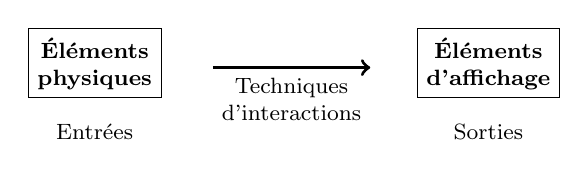
\begin{tikzpicture}[font=\footnotesize]
    \tikzstyle{label}=[below, align=center, text depth=.25ex]
    
    \draw (0,0) node[label, draw]{\textbf{Éléments}\\\textbf{physiques}};
    \draw (5,0) node[label, draw]{\textbf{Éléments}\\\textbf{d'affichage}};

    \draw[->, very thick] (1.5,-0.5) -- (3.5,-0.5)
      node[label, pos=0.5, below]{Techniques \\d'interactions};

    \draw (0,-1.1) node[label]{Entrées};
    \draw (5,-1.1) node[label]{Sorties};
  \end{tikzpicture}%
}{
  Principe d'une IHM : une technique interaction lie des entrées utilisateur, via un capteur physique, à un résultat affiché sur l'ordinateur.\\
  Adapté de \cite{Billinghurst2005}.
}

Une IHM constitue la principale interface avec laquelle un utilisateur va interagir avec un ordinateur. La bonne conception de cet intermédiaire est donc nécessaire pour rendre accessible et efficace le travail sur une machine. Son rôle est simple : comme le montre la \figref{Billinghurst2005}, il s'agit de lier des \emph{entrées utilisateurs} issues de capteurs physiques (souris, écran tactile, images d'une caméra) à des actions sur l'ordinateur représentées par un \emph{résultat en sortie} (affichage, son, commande) via une \emph{technique d'interaction} \citep{Billinghurst2005}. La technique d'interaction est donc \emph{une} méthode qui permet de traduire ces entrées en commandes : par exemple, le même mouvement avec une souris peut déplacer un curseur ou translater un objet le long d'un axe, ou encore un même déplacement de deux doigts sur un écran tactile peut faire une rotation ou un zoom sur un objet. Elle est également une métaphore qui permet à l'utilisateur d'associer ses actions avec des résultats sur l'ordinateur. Il existe de nombreux dispositifs d'entrée, de sortie et de techniques d'interaction, le défi étant de : \textquote{\texten{combine these together in a way that is most appropriate to the desired task, facilitates ease of use and learning and provides a high level of user performance and satisfaction}} \citep{Billinghurst2005}.

Un des but de la recherche en IHM est de réduire cet écart entre les éléments physiques et d'affichages \citep{VanDam1997}. \cite{Jacob2008} rappellent que les IHMs ont traversé plusieurs générations visant à chaque fois une utilisation plus simple, plus directe et plus proche des actions quotidiennes. Les ordinateurs s'utilisaient, avant les années 1960, par des cartes de commandes qui imprimaient alors leurs résultats. Puis ils ont été utilisés par ligne de commande via des terminaux jusque dans les années 1980. Enfin, les IHMs graphiques se sont démocratisées \figrefp{Jacob2008}, suivants le paradigme WIMP : un ensemble de fenêtres (\texten{windows}), d'icônes (\texten{icons}) et de menus (\texten{menus}) accessibles par un appareil de pointage (\texten{pointing device}), comme une souris. Ces IHMs sont excellentes pour des applications graphiques en 2D, mais limitées pour celles en 3D, entre autres\footnote{Les IHMs en ligne de commande sont toujours utilisées et complémentaires des IHMs graphiques : elles peuvent être plus puissantes et mieux adaptées que ces dernières, même si elles sont plus difficiles d'accès par le temps d'apprentissage qu'elles demandent.}. \cite{VanDam1997} appela alors à développer une nouvelle génération d'IHMs post-WIMP, c'est-à-dire contenant des techniques d'interactions non dépendantes de fenêtre, icônes ou de menu en 2D. L'objectif étant de diversifier les types d'IHMs pour proposer le plus adapté selon les besoins de l'utilisateur.

\figureETS[0.5]{Jacob2008}{
  Illustrations des deuxième (en ligne de commande) et troisième (par interface graphique WIMP) générations d'IHMs, ainsi que les nombreux types émergeants d'IHMs post-WIMP. Toutes sont complémentaires, chacune adaptée à des usages spécifiques qu'étudie la recherche sur les IHMs.\\
  Tiré de \cite{Jacob2008}.
}

Si de nombreuses IHMs post-WIMP ont par la suite été développées, comme celles désormais bien connues des téléphones intelligents à écrans tactiles \citep{Jacob2008}, aucun paradigme n'est encore établi pour la RA \citep{VanKrevelen2010}. \cite{Billinghurst2015} classent celles de RA en plusieurs catégories :
\begin{itemize}
  \item Navigateurs d'informations : affichant de l'information en RA sur l'environnement réel. Ce sont principalement les IHMs que l'on retrouve dans les applications pour téléphones intelligents \figrefp{MobileAR} : elles permettent simplement d'afficher du contenu en surimpression de l'environnement réel, l'utilisateur se déplaçant simplement pour le voir sous différents angles. Des IHMs WIMP sont souvent utilisées, mais ce type d'interfaces est limité dans les interactions avec le contenu virtuel en 3D.
  \item Interfaces en 3D : utilisant des techniques d'interactions en 3D pour manipuler le contenu dans l'espace.
  \item Interfaces tangibles : utilisant des objets réels pour interagir avec du contenu virtuel.
  \item Interfaces naturelles : utilisant les mouvements du corps de l'utilisateur, par exemple des commandes gestuelles.
  \item Interfaces multimodales : utilisant simultanément des commandes vocales et gestuelles.
\end{itemize}
\medskip

Pour \cite{Billinghurst2015}, toutes ces IHMs importent et appliquent des techniques d'interactions WIMP, de la RV ou des écrans tactiles. En ce sens, elles atteignent seulement les première et deuxième étapes du processus de \cite{Billinghurst2005} qui décrit les étapes de développement d'un paradigme d'IHM pour un nouveau média :
\begin{enumerate}
  \item développement de prototypes ;
  \item adoption de techniques d'interactions d'autres types d'IHM ;
  \item développement de métaphores et paradigmes d'IHMs adaptés au média ;
  \item développement de modèles théoriques pour ces paradigmes.
\end{enumerate}
\medskip

La RA présente pourtant un excellent média, car l'écart entre les éléments physiques et d'affichage (le contenu virtuel) y est très réduit. Cela permettrait de fondre la présence de l'ordinateur dans l'environnement de l'utilisateur sans le restreindre sur un écran. Une bonne IHM de RA permettrait alors de manipuler naturellement et efficacement du contenu virtuel en 3D avec des techniques d'interactions basées sur des objets physiques, des commandes vocales ou des gestes utilisés au quotidien \citep{Billinghurst2005}. C'est pourquoi il est important de consacrer un effort de recherche pour atteindre cette troisième étape, comme nous souhaitons le faire avec notre concept de téléphone à écran étendu, en utilisant des IHMs en 3D, les IHMs naturelles et les IHMs tangibles. Enfin, on remarque que la classification des IHMs de RA de \cite{Billinghurst2015} se concentre quasi exclusivement sur les techniques d'interactions. Pourtant, les données affichées ont toute leur importance, et il s'agit également de dépasser les concepts de fenêtre, menu et icônes des IHMs WIMP.

\subsection{IHMs en 3D et IHMs naturelles}
\label{subsec:litterature_ar_hci_interactions}

Les IHMs en 3D sont importées des recherches de la RV et dans les environnements virtuels (EV) en 3D. La recherche sur les EVs explore les interfaces et les interactions avec du contenu en 3D affiché sur un écran (et non de manière immersive comme en RA). \cite{Bowman2004} classent les techniques d'interactions en trois catégories : (1) navigation, (2) sélection (un ou plusieurs objets) et (3) manipulation (translation et rotation). Seules ces deux dernières sont applicables à la RA, le contenu virtuel étant aligné et intégré avec l'environnement réel, l'utilisateur se déplace simplement lui-même pour y naviguer.

De nombreux dispositifs d'entrée ont été développés pour les IHMs en 3D : des souris 3D, des joysticks, des stylos suivis en 3D ou des dispositifs haptiques (avec retour de force, donnant l'illusion de toucher le contenu virtuel). Tous permettent de sélectionner et manipuler avec précision du contenu virtuel ; on parle alors de degrés de libertés (\texten{degrees of freedom} ou DoF en anglais) pour caractériser les manipulations possibles, avec un degré par dimension donc maximum trois pour la translation et trois pour la rotation : une souris standard permet donc 2 DoFs, quand les dispositifs d'entrées des visiocasques de RV sont suivis avec 6 DoFs \figrefp{Evan-Amos2017}. Cependant, tous ces dispositifs présentent l'inconvénient d'occuper les mains de l'utilisateur : en RA, les espaces de visualisation et d'interaction sont donc séparés \figrefp{Adcock2003} et les techniques d'interactions avec les objets virtuels sont alors différentes de celles avec les objets réels \citep{Billinghurst2015}.

\figureLayoutETS{3DControllers}{%
  \subfigureETS[0.2]{Evan-Amos2017}{Les dispositifs d'entrée du visiocasque de RV Oculus Rift : sans fils, ils permettent de sélectionner du contenu virtuel et de le manipuler avec 6 DoFs.}%
  \figurehspace%
  \subfigureETS[0.2]{Adcock2003}{IHM de RA où la main gauche utilise plusieurs boutons pour interagir avec le menu 2D, tandis que la main droite tient un stylo haptique pour manipuler le crâne en 3D.}%
}{
  Exemples de dispositifs d'entrées pour IHMS en 3D.\\
  Tiré de a) \cite{Evan-Amos2017} et b) \cite{Adcock2003}.
}

Les IHMs naturelles utilisent quant à elle directement les mouvements du corps de l'utilisateur comme dispositif d'entrée, en particulier les mains. De nombreuses méthodes de vision par ordinateur permettent ce suivi en utilisant simplement les images d'une caméra \citep{Billinghurst2015}. Un utilisateur peut alors en théorie agir directement avec du contenu virtuel comme il le ferait avec des objets réels. Malgré tout, de telles interactions demandent souvent des mouvements complexes et fatigants à l'utilisateur \citep{Bowman2001}. De plus, ces IHMs ne peuvent répliquer exactement le monde réel : le manque de contraintes physiques rend les interactions imprécises \citep{Chan2010} et il peut être difficile de comprendre comment interagir avec un environnement virtuel utilisant une IHM naturelle \citep{Argelaguet2013}.

\figureLayoutETS{NaturalControllers}{%
  \subfigureETS[0.2]{Taylor2016}{Main virtuelle.}%
  \figurehspace%
  \subfigureETS[0.2]{Pfeuffer2017_1}{Pointeur virtuel.}%
}{
  Techniques d'interactions de sélection dans les IHMs naturelles.\\
  Tiré de a) \cite{Taylor2016} et b) \cite{Pfeuffer2017}.
}

Un écart existant donc toujours entre éléments physiques et éléments graphiques, des techniques d'interactions sont encore nécessaires. Deux types de techniques sont majoritairement utilisées. La \emph{main virtuelle} affiche un modèle 3D de main pouvant interagir avec le contenu virtuel et suivant la main réelle de l'utilisateur \figrefp{Taylor2016}. Elle est la plus naturelle, mais souffre particulièrement des problématiques que nous venons d'énoncer, mais aussi de problème d'occlusion, car elle peut cacher des objets virtuels. La technique du \emph{pointeur virtuel} permet à l'inverse de projeter un rayon, depuis la main ou la tête, pour sélectionner des objets \figrefp{Pfeuffer2017_1} : il permet d'atteindre facilement des objets lointains avec peu d'effort, mais cela est difficile s'ils sont de trop petite taille. De plus, si l'action de sélection peut entraîner un déplacement involontaire du pointeur, par exemple en pressant un bouton \citep{Argelaguet2013}. Cette technique a notamment été choisie pour le HoloLens : le pointeur suit les mouvements de la tête, stables et précis \citep{Kytoe2018}, tandis que la sélection se fait avec un geste de la main pour ne pas perturber le pointage.

La difficulté pour ce type d'IHM est donc de permettre des sélections et manipulations rapides, sans erreur ainsi que d'être faciles à comprendre et peu fatigantes \citep{Argelaguet2013}. Pour cela, il est crucial de fournir des retours à l'utilisateur : \cite{Chan2010} proposent la combinaison de retours continus, pour que l'utilisateur situe le suivi de son corps, et de retours discrets pour confirmer ses actions. Le modèle 3D de la main virtuelle avec des ombres portées ou le rayon du pointeur virtuel sont donc des retours visuels continus, tandis qu'un bref changement de couleur de l'objet peut confirmer une sélection. Ces retours ne doivent cependant pas être excessifs, au risque de produire une distraction et réduire la performance des utilisateurs \citep{Argelaguet2013}.

\figureETS[1]{Piumsomboon2013_1}{
  Les onze poses de mains utilisées pour des gestes en RA.\\
  Tiré de \cite{Piumsomboon2013}.
}

\figureETS[1]{Piumsomboon2013_2}{
  Extrait de la liste de gestes pour différentes tâches en RA. Les positions de mains utilisables sont indiquées entre crochets.\\
  Tiré de \cite{Piumsomboon2013}.
}

Si l'utilisation du pointeur virtuel telle qu'elle est faite par le HoloLens fonctionne bien \citep{Kytoe2018}, ce n'est pas le cas pour la main virtuelle dans les IHMs de RA malgré de nombreux prototypes \citep{Piumsomboon2013}. \cite{Piumsomboon2013} ont alors établi de manière rigoureuse une liste de gestes utilisables avec une main virtuelle en RA. Pour cela, ils ont tout d'abord montré des animations de quarante tâches courantes dans la littérature dans un visiocasque de RA à vingt participants et leur ont demandé de mimer en même temps que chaque animation le geste qu'ils utiliseraient. Ils ont alors sélectionné les poses de main les plus utilisées \figrefp{Piumsomboon2013_1}, ainsi que le ou les gestes majoritaires avec un score de consensus pour chaque tâche \figrefp{Piumsomboon2013_2}. Beaucoup de tâches ont un faible consensus (peu de participants ont utilisé le même geste), néanmoins ceux pour les menus ont un haut score $\geq 80\%$ \figrefp{Piumsomboon2013_3}. Enfin,la majorité de ces gestes sont réalisés \textquote{en l'air}, à l'exception de ceux ouvrant, fermant et sélectionnant un menu horizontal qui ont été réalisés sur la surface de la table \figrefp{Piumsomboon2013_2}.

\figureETS[0.9]{Piumsomboon2013_3}{
  Score de consensus sur le geste à utiliser (barres bleues) ainsi que ratio de gestes à deux mains (ligne rouge) parmi les participants pour chaque tâche.\\
  Tiré de \cite{Piumsomboon2013}.
}

Par la suite, \cite{Piumsomboon2014} ont comparé formellement quelques-unes de ces techniques avec des commandes vocales pour la sélection et la manipulation d'objets en 3D dans un visiocasque de RA. Leurs résultats indiquent que les participants étaient globalement plus rapides et préféraient utiliser des gestes pour manipuler les objets, mais des commandes vocales pour les redimensionner. Il serait cependant intéressant de reproduire cette étude avec des IHMs plus complexes que de simples objets 3D, par exemple avec des IHMs WIMP appliquées à la RA, comme le fait le HoloLens.

\figureLayoutETS{Piumsomboon2014}{%
  \subfigureETS[0.17]{Piumsomboon2014_1}{La main virtuelle fait occlusion avec le contenu 3D.}%
  \figurehspace%
  \subfigureETS[0.17]{Piumsomboon2014_2}{Le contenu 3D est transparent, laissant visible la main de l'utilisateur.}%
}{
  Différentes techniques d'occlusion de la main.\\
  Tiré de \cite{Piumsomboon2014}.
}

Enfin, \cite{Piumsomboon2013} et \cite{Piumsomboon2014} recommandent, à la suite d'études pilotes, que pour éviter les problèmes d'occlusion, les objets virtuels doivent toujours êtres visibles : soit en utilisant une main virtuelle transparente plutôt qu'opaque, soit en affichant leurs contours si elle les cache \figrefp{Piumsomboon2014}.

%TODO citer études avec mains virtuelles : \cite{Chan2010}, \cite{Markussen2014}, \cite{Hincapie-Ramos2014} et \cite{Jones2012}

\subsection{IHMs de RA tangibles}
\label{subsec:litterature_ar_hci_tui}

Les IHMs de RA tangibles utilisent des objets réels comme dispositifs d'entrées et d'affichages, qui sont alors augmentés par RA \citep{Kato2000}. Autrement dit, chaque objet virtuel est aligné avec un objet réel et est manipulé via cet objet réel \citep{Billinghurst2005} : les espaces d'interactions et d'affichage sont donc alignés et confondus. Ainsi, les interactions sont familières, faciles et intuitives et peuvent s'appuyer sur les contraintes physiques de ces objets réels \citep{Zhou2008}. Le principal inconvénient de ces IHM est de requérir des objets physiques, qui peuvent ne pas être présents dans l'environnement de l'utilisateur ou difficiles à transporter dans un usage mobile.

\figureLayoutETS{Lee2004}{%
  \subfigureETS[0.25]{Lee2004_1}{L'utilisateur presse les boutons du navigateur, puis créé l'objet courant en le pointant avec le cube de manipulation.}%
  \figurehspace%
  \subfigureETS[0.25]{Lee2004_2}{L'utilisateur déplace l'objet crée avec le cube, puis le fixe en cachant le haut du cube. Il le place dans la corbeille pour le détruire.}%
  \figurehspace%
  \subfigureETS[0.25]{Lee2004_3}{Redimensionnement d'un cube à l'aide d'un clavier connecté à un outil inspecteur affichant la propriété de taille du cube.}%
}{
  Exemple d'une IHM de RA tangible : les objets virtuels sont alignés avec des objets réels suivis avec 6 DoF et manipulés via des objets virtuels spécifiques utilisés comme outils.\\
  Tiré de \cite{Lee2004}.
}

Il existe toujours un écart entre entrées et affichages pour ce type d'IHM, en particulier pour certaines commandes : par exemple, pour changer les dimensions de l'objet virtuel ou, de manière générale, ses propriétés, l'activer ou encore réaliser des opérations de copie. Des techniques d'interactions sont donc toujours nécessaires, la difficulté étant de faire comprendre à l'utilisateur les commandes possibles et les conséquences de ces actions \citep{Zhou2008}. \cite{Lee2004} proposent par exemple d'utiliser certains objets réels comme des outils pour créer, détruire les autres objets virtuels ainsi que visualiser et modifier leurs propriétés : l'utilisateur place les outils proches des objets pour les faires interagir puis passe son doigt dessus comme pour effectuer un clic pour les activer \figrefp{Lee2004}.

Il existe deux approches pour concevoir une IHM de RA tangible : une seule fonction est attribuée à chaque outil dans une IHM à \emph{multiplexage spatial}, tandis qu'un même outil est utilisé pour plusieurs fonctions selon le contexte dans une IHM à \emph{multiplexage temporel} \cite{Billinghurst2015}. Le multiplexage spatial est plus facile à apprendre, mais le multiplexage temporel permet plus de flexibilité dans la conception de l'IHM. Par exemple, le cube de manipulation dans l'IHM de \cite{Lee2004} est à multiplexage spatial, car il a une seule fonction, tandis que l'outil inspecteur est à multiplexage temporel, car il affiche des données différentes en fonction de l'objet et de la propriété inspectés.

\figureLayoutETS{Lee2011}{%
  \subfigureETS[0.15]{Lee2011_1}{Navigateur d'information : le menu apparaît à distance fixe de l'utilisateur.}%
  \figurehspace%
  \subfigureETS[0.15]{Lee2011_2}{Tangible et aligné avec l'écran d'un téléphone tenu en main.}%
  \figurehspace%
  \subfigureETS[0.15]{Lee2011_3}{Tangible et aligné avec un objet de l'environnement.}%
}{
  Affichage d'un même menu selon différents types d'IHM de RA.\\
  Tiré de \cite{Lee2011}.
}

\figureLayoutETS{White2009}{%
  \parbox{0.965\textwidth}{%
    \centering%
    \subfigureETS[0.15]{White2009_1}{Quand le menu est activé, il est aligné avec un objet tenu en main.}%
    \figurehspace%
    \subfigureETS[0.15]{White2009_2}{Le menu peut alors rester tenu en main.}%
    \figurehspace%
    \subfigureETS[0.15]{White2009_3}{Le menu peut rester attaché à la tête de l'utilisateur.}%
    \\%
    \subfigureETS[0.15]{White2009_4}{Le menu peut rester fixe dans l'espace.}%
    \figurehspace%
    \subfigureETS[0.15]{White2009_5}{Le menu peut être attaché à une planche : la sélection est alors bi-manuelle.}%
    \figurehspace%
    \subfigureETS[0.15]{White2009_6}{La sélection d'un élément du menu se fait en le pointant avec l'objet tenu en main.}%
  }%
}{
  Différents placements possibles d'un menu de RA.\\
  Tiré de \cite{White2009}.
}

Un téléphone peut donc être utilisé comme base d'IHM de RA tangible, par exemple pour afficher des menus alignés avec l'écran \figrefp{Lee2011}. \cite{White2009} ont comparé l'usage d'un tel menu aligné avec d'autres placements possibles, par rapport à la tête de l'utilisateur ou par rapport à l'environnement \figrefp{White2009}. L'utilisateur sélectionne un élément du menu en le pointant avec l'objet tenu en main. Dans les résultats de leur étude expérimentale, où treize participants ont effectué chacun 80 sélections avec chaque type de menu, leurs résultats indiquent que les sélections ont été statistiquement plus rapides dans les cas du menu tenu en main ou attaché à la tête de l'utilisateur (en moyenne en \SI{3}{\s} contre \SIrange{7}{8}{\s}). Les utilisateurs ont également préféré ces deux techniques. Pour les auteurs, ces deux conditions étaient les plus stables et les plus faciles à utiliser. Pourtant le menu attaché à la main est plus intéressant car l'utilisateur peut facilement le déplacer ou changer son orientation. Cette étude supporte donc la faisabilité d'une IHM de RA tangible basée sur un téléphone tenu en main.

\subsection{Évaluation d'IHM en RA}
\label{subsec:litterature_ar_hci_evaluation}

Pour déterminer si une IHM est fonctionnelle et pertinente, on peut l'évaluer avec des études utilisateurs \citep{Billinghurst2015}. Cela permet de mesurer efficacement l'utilisabilité de l'interface, les résultats obtenus permettent en outre de donner des clés de conception à d'autres chercheurs dans le domaine ainsi qu'à des concepteurs et développeurs \citep{Jankowski2015}. Enfin, correctement décrites, ces études peuvent également être répliquées et leurs résultats vérifiés et discutés indépendamment.

Concrètement, plusieurs personnes sont recrutées pour utiliser différents systèmes (par exemple des IHMs) de RA dans différentes configurations sur une même tâche. L'objectif est alors d'évaluer et comparer ces systèmes et configurations, et non pas les utilisateurs. On cherche alors à répondre à des questions sur ces systèmes et leur usage ; on conçoit alors la tâche et des mesures pour obtenir des données pour répondre à ces questions. \cite{Swan2005} et \cite{Duenser2008} catégorisent les études utilisateurs en RA selon les questions qu'elles visent : (1) perception et cognition humaine, (2) interactions et (3) communication et collaboration. Seule une minorité des articles contenaient alors une étude utilisateur (environ 10\%), la plus grande part d'entre elles étant consacrées aux interactions en RA.

\cite{Duenser2008} ont recensés différents types de mesures utilisées dans les études utilisateurs en RA :
\begin{enumerate}
  \item \emph{Mesures objectives} : ce sont les mesures de performance, comme le temps de complétion de la tâche, le nombre d'erreurs, la précision, les mouvements effectués ou encore le nombre d'actions. Des analyses statistiques sont ensuite fréquemment employées pour agréger et décrire les données. Ces mesures sont couramment utilisées.
  \item \emph{Mesures subjectives} : ce sont des mesures faites par les utilisateurs via des questionnaires, des notes et commentaires. Des analyses statistiques sont aussi utilisées, mais parfois seule une description des résultats est faite. Ces mesures sont assez souvent utilisées. De nombreux outils existent pour mesurer la charge de travail subjective d'une IHM, comme le NASA-TLX \citep{Rubio2004}.
  \item \emph{Analyses qualitatives} : elles correspondent à des observations utilisateurs, des entrevues formelles, ou encore à une classification des comportements utilisateurs. Ces mesures sont assez peu utilisées.
  \item \emph{Évaluation d'utilisabilité} : utilisation de techniques comme des évaluations heuristiques, des évaluations d'experts, des analyses de tâche. La méthode du magicien d'Oz est une simulation d'IHM, où l'utilisateur simule ces actions et le chercheur simule les résultats, par exemple à l'aide d'éléments d'interface faits en cartons. Une dernière technique est de demander à l'utilisateur de décrire à voix hautes ces actions et réactions par rapport au système de RA. Ces techniques sont assez peu utilisées.
  \item \emph{Évaluations informelles} : ce sont des observations informelles d'utilisateurs ou des retours utilisateurs informels. Cela est utile pour des études pilotes ou pour donner des pistes de réponses sur le système de RA. Ces méthodes sont couramment utilisées.
\end{enumerate}

Des analyses statistiques permettent de comprendre et interpréter des données mesurées. En pratique, on cherche souvent à indiquer des différences entre différents systèmes de RA, par exemple que les utilisateurs sont plus performants sur une IHM qu'avec une autre. On dit alors qu'une des IHM a un effet sur la performance (temps, erreurs) par rapport à l'autre. Or, on a pris des mesures que sur un \emph{échantillon} de la \emph{population}, qu'on espère suffisamment représentatif. On peut analyser les mesures de l'échantillon, mais on souhaiterait pouvoir dire avec un certain niveau de confiance que les résultats sont également applicables à la population.

Le test de l'hypothèse nulle est souvent utilisé pour cela dans la littérature en IHM. On postule une hypothèse alternative qu'on nomme l'hypothèse nulle : par exemple, il n'y a pas de différence d'effet sur la performance des utilisateurs entre les deux IHMs. On calcule alors la probabilité, la \emph{valeur-p}, d'observer de tels résultats s'il n'y avait en réalité pas d'effet (si l'hypothèse nulle est vraie). Typiquement, on se donne 5\% de chance d'erreur, c'est-à-dire qu'on considère que si $p < 0.05$ alors on peut rejeter l'hypothèse nulle et dire qu'il y a un effet \emph{statistiquement significatif} : on considère que ce serait trop improbable d'obtenir de tels résultats s'il n'y avait pas d'effet. La valeur-p n'est cependant \emph{pas} la probabilité qu'il n'y ait pas d'effet.

\figureLayoutETS{Dragicevic2016}{%
  \subfigureETS[0.25]{Dragicevic2016_1}{Moyennes de l'effet sur le poids de pilules amaigrissantes imaginaires, avec valeurs-p et intervalles de confiance.}%
  \figurehspace%
  \subfigureETS[0.25]{Dragicevic2016_2}{Valeurs-p et intervalles de confiance de la moyenne d'échantillons (taille = 25) tirés d'une population normallement distribuée (moyenne = 10, écart-type = 20).}%
}{
  Comparaison des valeurs-p et des intervalles de confiance (sous forme de barres d'erreurs) sur des résultats.\\
  Adapté de \cite{Dragicevic2016}.
}

Pourtant cette pratique est controversée. Premièrement, si on se donne une chance d'erreur sur chaque test, plus on effectuera de tests, plus on aura de chance d'avoir rejeté à tord l'hypothèse nulle sur un des tests : c'est le problème des comparaisons multiples. Ainsi, pour $20$ tests, on a probablement déclaré $20 \times 0.05 = 1$ effet significatif alors qu'il n'y a en réalité pas (par exemple, échantillons 4 et 7 dans la \figref{Dragicevic2016_2}). En pratique, il est cependant possible de réduire ou contrôler ce risque à l'aide de méthodes de correction (Holm-Bonferroni ou Benjamini-Hochberg par exemple). Deuxièmement, on ne sait pas la taille de l'effet en lui-même, ni on ne peut conclure quoi que ce soit si la valeur-p est trop élevée (par exemple, pilule 2 dans la \figref{Dragicevic2016_1}).

\cite{Dragicevic2016} propose alors de remplacer les tests de l'hypothèse nulle avec le calcul d'\emph{intervalles de confiance} (IC) : c'est une marge d'erreur autour d'une estimation de l'échantillon, par exemple une moyenne, avec un degré de confiance fixé, typiquement typiquement 95\%. Plus précisément, un intervalle de confiance à 95\% contiendra 95 fois sur 100 l'estimation de la population (par exemple, on ne capture pas la moyenne de la population avec les échantillon 7 et 17 dans la \figref{Dragicevic2016_2}). En pratique, on peut donc le considérer comme l'intervalle des valeurs les plus plausibles de l'estimation. Ainsi, en comparant les intervalles de confiance de deux mesures, on détermine \emph{l'importance significative} de l'effet.

Dès lors, on peut considérer que la valeur-p et l'intervalle de confiance donnent en pratique la même information \cite{Dragicevic2016}. Cependant, le test de l'hypothèse nulle est couramment utilisé dans la littérature en IHM. C'est pourquoi nous avons choisis de le conserver et de l'utiliser conjointement à des intervalles de confiances à 95\%.


\section{Espaces de travail en RA}
\label{sec:litterature_ar_worspaces}

La séparation entre les styles d'IHMs faite par \cite{Rekimoto1995} \figrefp{Rekimoto1995} est artificielle : pour \cite{Billinghurst2005} la RA devrait s'intégrer avec l'informatique ubiquitaire, les IHMs graphiques et la RV. Par exemple, \cite{Heun2013} utilise la RA comme interface pour interagir de façon naturelle avec les objets intelligents autour de soi \figrefp{Heun2016}, tandis que le prototype SpaceTop de \cite{Lee2013} permet de placer les fenêtres d'une IHM WIMP sur une grille en 3D \figrefp{Lee2013}.

\figureETS[0.7]{Heun2016}{
  Photographie du \texten{Reality Editor}, un navigateur web de RA pour interagir facilement avec les objets intelligents autour de soi. Ici, une personne paye un parc-mètre via son téléphone.\\
  Tiré de \cite{Heun2013}.
}

Google Glass a été une expérience novatrice de visiocasque de RA. Malgré les problèmes de vie privée et d'acceptation sociale que son usage a posé, \cite{Koelle2015} rappellent que cela a montré qu'il était intéressant de combiner un visiocasque de RA avec un téléphone intelligent. L'utilisateur interagissait avec son téléphone via le visiocasque, par des interactions multimodales à la voix ou encore avec des gestes en l'air décodés par la caméra du visiocasque. Cette expérience montre ainsi que les visiocasques de RA vont d'abord prendre place dans nos quotidiens professionnels où ils seront mieux acceptés ; c'est également la stratégie de la nouvelle version de ce visiocasque \cite{Levy2017}. Il est donc plus intéressant d'orienter des recherches en IHM pour la RA.

Le Google Glass était un prototype limité visible seulement par l'\oe il droit avec un faible champ de vision \figrefp{Phandroid2013_1}. Mais surtout, il ne proposait pas une véritable IHM de RA : affichée sur un unique plan virtuel à une distance fixe des yeux de l'utilisateur \figrefp{Phandroid2013_2}, comme sur la \figref{White2009_3}, elle ne répond pas à l'alignement virtuel-réel dans la définition d'\cite{Azuma1997}. Aussi, cette fenêtre virtuelle peut faire occlusion avec l'environnement réel, et gêner la vue de l'utilisateur. De nombreux autres visiocasques, comme Epson Moverio ou Vusix, souffrent de ces mêmes limites. C'est pourquoi le HoloLens a apporté une innovation majeure dans l'industrie de la RA en proposant de placer de multiples fenêtres virtuelles contre les murs, comme on peut accrocher un tableau, donnant réellement le sentiment qu'elles font partie de l'environnement réel.

\figureLayoutETS{Glass}{%
  \subfigureETS[0.2]{Phandroid2013_1}{Utilisateur portant le visiocasque : le champ de vision est très petit et limité à l'\oe il droit.}%
  \figurehspace%
  \subfigureETS[0.2]{Phandroid2013_2}{Vue depuis le visiocasque : l'IHM est affichée sur un rectangle à distance fixe de l'utilisateur sans intégration avec l'environnement réel.}%
}{
  Photographies du Google Glass.\\
  Tiré de \cite{Phandroid2013}.
}

Partant de la même limite d'un seul écran de ces visiocasques, \cite{Ens2014} proposent alors le Personal Cockpit, une IHM de RA affichant de multiples fenêtres autour de l'utilisateur \figrefp{Ens2014}. Il peut y organiser l'information sur différents écrans qui le suivent dans ces déplacements et avec qu'il interagit directement avec une technique de main virtuelle. Les auteurs mesurent alors qu'un utilisateur travaille 40\% plus rapidement avec de multiples fenêtres qu'avec une simple fenêtre fixe en faisant du multi-tâches. Ils y évaluent également plusieurs facteurs de conception : leurs résultats indiquent (1) qu'un affichage courbe est moins fatiguant et moins sujet à des erreurs de sélection, les fenêtres étant ainsi affichées à la même distance de l'utilisateur, (2) que les interactions avec une main virtuelle sont plus stables et faciles avec des fenêtres fixées dans l'espace que placées sur le corps, car l'utilisateur peut les faire bouger involontairement, et (3) que la distance minimum des fenêtres est à \SI{50}{\cm} de l'utilisateur, provoquant autrement de l'inconfort. Cependant, leur étude utilisait un CAVE simulant un petit champ de vision de $\ang{40} \times \ang{30}$ : il serait alors intéressant de la reproduire avec visiocasque à large champ de vision.

\figureLayoutETS{Ens2014}{%
  \subfigureETS[0.12]{Ens2014_1}{Positionnement idéal des fenêtres virtuelles en un affichage courbe.}%
  \figurehspace%
  \subfigureETS[0.12]{Ens2014_2}{Exemple d'utilisation avec une carte de navigation.}%
}{
  Photographies et illustrations du Personal Cockpit.\\
  Tiré de \cite{Ens2014}.
}

Avec MultiFi, \cite{Grubert2015} explorent de leur côté comment combiner les entrées et les sorties des appareils intelligents que nous portons (téléphone, tablettes, montre) avec un visiocasque de RA. Ces appareils mobiles ne sont souvent pas conçus pour travailler ensemble, mais gagneraient à l'être. La \figref{Grubert2015_2} montre par exemple une liste affichée sur une montre à l'écran étendu : en plaçant son téléphone sur un élément de la liste, l'utilisateur peut alors le voir en détails. Les différentes tailles et définitions d'affichage sont ainsi exploitées pour composer une seule vue pour l'utilisateur.  Les auteurs distinguent alors trois alignements possibles entre une fenêtre virtuelle de RA et un appareil mobile \figrefp{Grubert2015_1} :
\begin{enumerate}
  \item mode \texten{body-aligned} : la fenêtre a pour référence le corps de l'utilisateur, comme \cite{Ens2014}, l'appareil mobile formant alors une vue \texten{detail} sur le contenu (\figref{Grubert2015_3}, similaire à \cite{Berge2014}) ;
  \item mode \texten{device-aligned} : la fenêtre est centrée et alignée sur l'appareil mobile dont elle étend l'écran \figrefp{Grubert2015_2} ;
  \item mode \texten{side-by-side} : un des appareils, visiocasque compris, redirige ces interactions vers un autre appareil, par exemple les interactions tactiles du téléphone vers une fenêtre virtuelle.
\end{enumerate}
\medskip

\figureETS{Grubert2015_1}{
  Illustrations des alignements possibles de contenu entre un visiocasque de RA et un appareil mobile : le mode \texten{body-aligned} à gauche, le mode \texten{device-aligned} au milieu et le mode \texten{side-by-side} à droite.\\
  Tiré de \cite{Grubert2015}.
}

Leurs résultats expérimentaux, dans une tâche de recherche d'information et de pointage, montrent que le couplage des appareils mobiles avec un visiocasque de RA peut permettre des temps plus rapides par rapport aux appareils seuls, visiocasque compris, mais au détriment d'un plus grand effort perçu par les utilisateurs. En outre, les préférences des utilisateurs étaient variées, ce qui montre que le choix du couplage entre appareils mobiles et visiocasque doit être laissé à l'utilisateur. Cependant, le visiocasque utilisé était lourd et avait aussi un petit champ de vision de $\ang{31} \times \ang{17}$ : ne pouvant pas voir de large contenu en une fois, les participants devaient fréquemment bouger la tête. De plus, seules des interactions sur les écrans tactiles, ou en plaçant l'appareil mobile dans l'espace, ont été évaluées. Il serait intéressant de les comparer avec des interactions utilisant une main virtuelle, et dans un visiocasque avec un large champ de vision.

\figureLayoutETS{Grubert2015_Demos}{%
  \subfigureETS[0.16]{Grubert2015_2}{Une montre intelligente à écran étendu par RA en haut (mode \texten{device-aligned}). Un téléphone intelligent placé sur la partie virtuelle de l'écran étendu (vue \texten{overview}) permet de le voir plus détaillé (vue \texten{detail}).}%
  \figurehspace%
  \subfigureETS[0.16]{Grubert2015_3}{L'utilisateur pointe son téléphone vers des éléments affichés par le visiocasque en mode \texten{body-aligned} pour les voir en détail.}%
  \figurehspace%
  \subfigureETS[0.16]{Grubert2015_4}{L'écran haute résolution (vue \texten{focus}) d'une montre intelligente étendu par le visiocasque de plus basse résolution (vue \texten{context}).}%
}{
  Démonstrations de MultiFi.\\
  Tiré de \cite{Grubert2015}.
}

\cite{Serrano2015} généralisent avec Gluey le mode \texten{side-by-side} de MultiFi. Un visiocasque de RA affichant du contenu virtuel en permanence sans encombrer les mains de son utilisateur est le support idéal pour transmettre de l'information facilement entre différents appareils. Par exemple, une personne peut utiliser un clavier, une souris ou un écran tactile et voir ses actions s'exécuter sur un autre appareil qu'il regarde \figrefp{Serrano2015_1}, ou encore copier des données depuis un ordinateur et les \textquote{coller} sur une imprimante pour les imprimer \figrefp{Serrano2015_Demos}. Pour les auteurs, les fonctionnalités d'une telle IHM sont (1) la redirection des entrées entre les appareils, (2) la migration du contenu entre les appareils, (3) la compatibilité de tous les appareils pour 1 et 2, (4) l'identification des appareils disponibles, (5) l'identification de leurs positions, (6) donner des retours de ces actions à l'utilisateur et (7) être mobile. Ainsi, MultiFi ne satisfait qu'aux critères 1, 5, 6 et 7. Cet article présente toutefois des limites par la faiblesse de son évaluation informelle mais aussi par le faible champ de vision de leur visiocasque.

\figureETS[1]{Serrano2015_1}{
  Illustration du concept de Gluey : le visiocasque de RA sert de support intermédiaire pour transmettre de l'information facilement entre tous les appareils disponibles.\\
  Tiré de \cite{Serrano2015}.
}

\figureLayoutETS{Serrano2015_Demos}{%
  \subfigureETS[0.3]{Serrano2015_2}{Copie du lien d'une vidéo vers le presse-papier du visiocasque.}%
  \figurehspace[2]%
  \subfigureETS[0.3]{Serrano2015_3}{Impression d'une image en la déplaçant du presse-papier du visiocasque pour la déposer sur l'imprimante.}%
}{
  Démonstration de Gluey.\\
  Adapté de \cite{Serrano2015}.
}

Enfin, \cite{Serrano2015a} ont complété Gluey en proposant un concept de \emph{bureau virtuel} qu'ils ont nommé Desktop-Gluey. Cette série d'IHMs permet d'intégrer des fenêtres virtuelles dans un environnement de travail de bureau. Leur première idée est de les utiliser en parallèle d'écrans d'ordinateur voire de les remplacer tout en continuant à utiliser clavier et souris, comme avec Gluey \figrefp{Serrano2015a_1}. Ces fenêtres virtuelles peuvent également être placées pour étendre des écrans physiques comme dans le mode \texten{device-aligned} de MultiFi ou dans des dispositions spatiales similaires au Personal Cockpit \figrefp{Serrano2015a_2}. Enfin, le bureau virtuel peut être emmené avec soi, en utilisant son téléphone ou une tablette pour interagir avec ou par des interactions directes utilisant une main virtuelle \figrefp{Serrano2015a_3}. Ce court article ne présente en revanche ni prototype ni d'évaluation expérimentale.

\figureLayoutETS{Serrano2015a_Demos}{%
  \subfigureETS[0.14]{Serrano2015a_1}{Les fenêtres virtuelles peuvent remplacer des écrans physiques, tout en continuant à utiliser clavier et souris, comme dans Gluey.}%
  \figurehspace%
  \subfigureETS[0.14]{Serrano2015a_2}{Les fenêtres virtuelles peuvent étendre des écrans physiques.}%
  \figurehspace%
  \subfigureETS[0.14]{Serrano2015a_3}{En mode mobile, les fenêtres suivent l'utilisateur comme dans le Personal Cockpit.}%
}{
  Illustrations de Desktop-Gluey : ce concept de bureau virtuel explore comment les fenêtres virtuelles vue par RA peuvent s'intégrer dans un espace de travail de bureau.\\
  Adapté de \cite{Serrano2015}.
}

On peut mieux comprendre comment toutes ces IHMs s'articulent entre elles en utilisant le cadre de conception Ethereal Planes \citep{Ens2014a}. Il permet de classer et concevoir les IHMs de RA utilisant des fenêtres 2D selon sept dimensions :
\begin{itemize}
  \item Cadre de référence :
  \begin{itemize}
    \item \emph{Perspective} : les fenêtres sont placées par rapport au corps ou à la tête de l'utilisateur (\emph{égocentrique}) ou par rapport à l'environnement (\emph{exocentrique}).
    \item \emph{Mobilité} : les fenêtres sont \emph{mobiles} ou \emph{fixes}.
    \item \emph{Proximité} : la distance avec l'utilisateur, \emph{sur le corps}, à portée de main (\emph{proche}) ou au-delà (\emph{lointain}).
  \end{itemize}
\end{itemize}
\newpage % Pour ne pas couper la sous-liste ci-dessous, TODO ajustement à vérifier à chaque modification de ce chapitre
\begin{itemize}
  \item Manipulation spatiale :
  \begin{itemize}
    \item \emph{Mode d'entrée} : les techniques d'interactions sont soit \emph{directes} (écran tactile, main virtuelle), soit \emph{indirectes} (pointeur virtuel).
    \item \emph{Tangibilité} : les techniques d'interactions sont \emph{tangibles} ou \emph{intangibles}.
  \end{itemize}
  \item Composition spatiale :
  \begin{itemize}
    \item \emph{Visibilité} : si le contenu est visible (\emph{haut}), par exemple avec un grand champ de vision, ou s'appuie sur la mémoire spatiale de l'utilisateur (\emph{bas}).
    \item \emph{Discrétisation} : décrit la fragmentation de l'espace virtuel, qui est plutôt \emph{continu} (un seul affichage) ou \emph{discret} (de multiples affichages disjoints).
  \end{itemize}
\end{itemize}
\medskip

Par exemple, \cite{Ens2014a} évaluent leur Personal Cockpit comme égocentrique et mobile, proche de l'utilisateur, à interactions indirectes et intangibles, avec une petite visibilité et continu (les écrans forment une \textquote{bulle} continue autour de l'utilisateur). Ils classent de la même manière un échantillon de 34 IHMs dans la littérature dans leur cadre en cinq catégories \figrefp{Ens2014a}. Par exemple, les applications de RA sur mobile, où la RA est vue à travers le téléphone tenu en main font partie de la catégorie \texten{peephole}, tandis que le HoloLens fait partie de la catégorie \texten{floating} où des fenêtres virtuelles sont placées par rapport aux murs. Ce cadre est également utile pour décrire plusieurs modes d'une IHM : un utilisateur de Desktop-Gluey place par exemple les fenêtres autour d'écran d'ordinateur dans un cadre alors exocentrique et fixé, ou autour d'un téléphone tenu en main dans un cadre égocentrique et mobile.

\figureETS[1]{Ens2014a}{
  Application du cadre de conception \texten{Ethereal Planes} à quelques exemples dans la littérature regroupés en cinq catégories.\\
  Tiré de \cite{Ens2014a}.
}

On pourrait s'étonner que toutes ces IHMs que nous venons de voir se limitent à des fenêtres 2D pourtant affichées dans un espace en 3D. \cite{Ens2014a} indiquent que nous devons déjà comprendre comment concevoir des affichages 2D en RA, car ils sont connus et bien maîtrisés sur les ordinateurs (IHMs WIMP), les téléphones ou montres intelligents et permettent donc de travailler rapidement et avec précision. De plus, les affichages 2D resteront toujours présents sous forme d'IHM et même physiquement, car [traduction] \textquote{ils resteront adaptés pour un large éventail d'utilisations, particulièrement celles impliquant des simplifications ou abstractions d'informations (par exemple, du texte, des plans, des panneaux de contrôles)} \citep{Ens2014a}. De plus, l'étude d'affichages 2D en RA reste intéressante, car elle exclue des problématiques spécifiques aux IHMs 3D, comme l'occlusion ou la difficulté de s'orienter \citep{Berge2014}, et permet ainsi de se concentrer sur comment présenter l'information et comment interagir avec. Toutes ces IHMs et ce cadre de conceptions sont donc une passerelle pour ensuite bâtir des IHMs spécifiques à la RA (troisième étape du processus de \cite{Billinghurst2005}).


\section{IHMs multi-échelles et larges affichages}
\label{sec:litterature_multiscale_displays}

\figureLayoutETS{Guiard2004Document}{%
  \subfigureETS[0.4]{Guiard2004_1}{La vue de l'écran sur le document représentée par un rectangle noir.}%
  \figurehspace%
  \subfigureETS[0.4]{Guiard2004_2}{Le document représenté à différents niveaux d'échelle, le long de l'axe S, la vue restant de taille constante.}%
  \figurehspace%
  \subfigureETS[0.4]{Guiard2004_3}{Vues du document à différentes échelles.}%
}{
  Visualisation d'un large document sur un écran plus petit.\\
  Adapté de \cite{Guiard2004}.
}

Dépasser les limites physiques d'un écran est un thème courant dans la littérature. En effet, à partir des années 1990, les écrans des PCs ont été largement dépassés en taille par celle de certains documents \citep{Guiard2004}. Ces documents peuvent être des cartes géographiques, des plans, de la création graphique ; l'écran manquant de pixels (basse définition)\footnotemark\ ou étant trop petit, il n'est alors pas possible de travailler correctement avec, car il est impossible visualiser en même temps une vue des détails et une vue d'ensemble \figrefp{Guiard2004Document}. En outre, \cite{Guiard2004} montrent que la difficulté pour naviguer dans un grand document est inversement proportionnelle à la taille de l'écran (jusqu'à une certain seuil de taille). De même, un écran virtuel en RA de petite taille complique le multi-tâche \citep{Ens2014}. De manière plus générale, toute information ou IHM doit tenir compte des limites de l'écran sur laquelle elle est affichée car, même si un affichage parfait existait, il serait limité par le champ de vision et la résolution de l'œil humain \citep{Cockburn2008}.

\footnotetext{La résolution d'un écran, en pixels par pouce, permet de convertir sa définition $(d_x,d_y)$, en pixels, vers sa taille physique $(L,H)$, en centimètres, et vice-versa : 
$\left\{
  \begin{array}{l}
    L = d_x/resolution\\
    H = d_y/resolution
  \end{array}
\right.$.}

\figureLayoutETS{Guiard2004Techniques}{%
  \subfigureETS[0.2]{Guiard2004_4}{Pan+Zoom : permet de défiler et zoomer à travers une seule vue dans le document.}%
  \figurehspace%
  \subfigureETS[0.2]{Guiard2004_5}{Overview+Detail : affiche simultanément une vue zoomée et une vue du document entier.}%
  \figurehspace%
  \subfigureETS[0.2]{Guiard2004_6}{Focus+Context : affiche une vue du document entier et un zoom par une distorsion optique (sphérique à gauche et linéaire à droite).}%
}{
  Techniques de visualisation et de navigation d'un large document sur un écran plus petit.\\
  Adapté de \cite{Guiard2004}.
}

\figureLayoutETS{MultiscaleDisplayExemples}{%
  \subfigureETS[0.22]{Burigat2013}{Exemple d'IHM Overview+Detail avec une carte de navigation : une vue du document entier (en bas à droite) est affichée par-dessus une vue zoomée.}%
  \figurehspace%
  \subfigureETS[0.22]{Guiard2004_7}{Exemple d'IHM Focus+Context avec une distorsion optique sphérique à gauche et linéaire à droite.}%
}{
  Exemples des techniques a) Overview+Detail et b) Focus+Context.\\
  Adapté de a) \cite{Burigat2013} et b) \cite{Guiard2004}.
}

Une approche à ce problème est d'utiliser des IHMs multi-échelles (\texten{multiscale interfaces} en anglais). Le principe est d'afficher à l'écran une ou plusieurs \emph{vues} du document à différentes échelles et positions. \cite{Guiard2004} décrivent trois techniques courantes :
\begin{itemize}
  \item Pan+Zoom : une vue peut-être déplacée sur le document par défilement (\texten{pan}), tandis que le zoom permet de changer l'échelle du document \figrefp{Guiard2004_4}. Il y a donc une séparation temporelle entre les vues.
  \item Overview+Detail : une vue zoomée (\texten{detail}) et une vue sur le document en entier (\texten{overview}) sont affichées simultanément \figrefp{Guiard2004_5}, créant une séparation spatiale de l'affichage. Elles sont placées côte-à-côte ou superposées et peuvent être déplacées indépendamment \figrefp{Burigat2013}.
  \item Focus+Context : une seule vue permet d'afficher le document en entier et le document zoomé \figrefp{Guiard2004_6}, par exemple grâce à une distorsion optique \figrefp{Guiard2004_7}.
\end{itemize}
\medskip

\cite{Cockburn2008} y ajoutent une quatrième technique : les indications visuelles. Cela consiste à modifier le document pour pointer certaines informations, par exemple en les surlignant, en modifiant leur taille ou encore en effaçant les informations moins importantes. Elles ont toutes été étudiées exhaustivement. Pourtant, aucune n'est idéale : l'utilisateur doit comprendre la séparation temporelle de la vue pour Pan+Zoom ou la séparation spatiale, qui ne doit alors pas être trop importante entre les deux vues, pour Overview+Detail et la distorsion Focus+Context nuit à la performance dans les tâches de sélections \citep{Cockburn2008}. Enfin, ces quatre techniques sont compatibles : beaucoup d'applications utilisent la combinaison Pan+Zoom, Overview+Detail avec des indications visuelles.

Une autre approche, complémentaire aux IHMs multi-échelles, est donc d'augmenter la taille et la définition de l'écran. \cite{Baudisch2002} ont par exemple agrandit un écran d'ordinateur par un projecteur : cette combinaison forme une IHM Focus+Context, le projecteur ayant une résolution beaucoup plus réduite que celle de l'écran \figrefp{Baudisch2002}. Comparé à des IHMs sur ordinateur Pan+Zoom et Overview+Detail dans une étude utilisateur avec deux tâches de navigation (une carte et un plan de circuit électronique), leur prototype est 21\% à 36\% plus rapide. Cela est dû probablement à sa grande taille qui permet, malgré sa faible résolution, à un utilisateur de reconstruire plus facilement une image mentale du document.

\figureETS[0.5]{Baudisch2002}{
  Combinaison d'un écran d'ordinateur haute résolution (\texten{focus}) aligné avec un projecteur basse résolution (\texten{context}).\\
  Tiré de \cite{Baudisch2002}.
}

\figureETS[0.5]{Andrews2010}{
  Large affichage d'une définition de \SI{10240x3200}{\px} composé de \num{4x2} écrans.\\
  Tiré de \cite{Andrews2010}.
}

\cite{Czerwinski2003} se demandent alors si de plus grands écrans hautes résolutions mènent à de même résultats pour des activités multi-tâches. Ils comparent alors un unique écran de 15 pouces avec un affichage courbe composé de multiples écrans (équivalent à trois écrans de 15 pouces côte-à-côte), dans une étude utilisateur demandant de travailler sur une tâche complexe avec de multiples fenêtres. La \figref{Andrews2010} montre un exemple similaire d'affichage de plusieurs écrans. Leurs résultats indiquent que les participants sont significativement (9\%) plus rapides avec l'affichage large et le préfèrent. Les auteurs ont observé que les utilisateurs perdaient du temps sur le petit écran à faire la gestion des fenêtres (changement de taille, repositionnement). Cependant, le grand affichage demandait un temps d'apprentissage, car il leur était inhabituel.

\figureLayoutETS{Mehra2006}{%
  \subfigureETS[0.15]{Mehra2006_1}{Vue initiale.}%
  \figurehspace%
  \subfigureETS[0.15]{Mehra2006_2}{Défilement statique : l'utilisateur déplace le document (l'écran reste fixe).}%
  \figurehspace%
  \subfigureETS[0.15]{Mehra2006_3}{Défilement dynamique : l'utilisateur déplace l'écran (le document reste fixe).}%
}{
  Différents types de défilement d'un large document. Le rectangle gris représente le document, le carré blanc l'écran.\\
  Adapté de \cite{Mehra2006}.
}

Les techniques des IHMs multi-échelles requièrent toutes des opérations de défilements de la part de l'utilisateur. \cite{Mehra2006} distinguent deux types de défilements : statiques, où l'utilisateur déplace le document tandis que l'écran reste fixe \figrefp{Mehra2006_2}, ou dynamiques, où l'utilisateur déplace l'écran tandis que le document reste fixe \figrefp{Mehra2006_3}. L'avantage pour ce second type de défilement est que l'utilisateur peut se servir de sa mémoire spatiale pour se construire une représentation du document. Dans une étude utilisateur, \citeauthor{Mehra2006} comparent les deux types de défilement : les participants ont navigué sur un écran par défilement à l'aide d'une souris dans un document affichant des lignes pour déterminer la plus grande \figrefp{Mehra2006}. Les réponses correctes et les temps de réactions sont meilleurs avec un défilement dynamique qui est également préféré des participants. Pour \citeauthor{Mehra2006}, une personne utilisant le défilement dynamique a simplement à reconstruire le document à travers le temps, les lignes restant fixes par rapport à lui. Au contraire, un défilement statique demande plus d'effort avec une reconstruction du document à la fois à travers le temps et à travers l'espace, les lignes changeant de positions \figrefp{Mehra2006_2}.

Dans la continuité des études sur la taille, le nombre et la résolution des écrans sur ordinateurs, beaucoup d'études sont faites sur les affichages muraux. Ces grands affichages ont suffisamment de définition pour afficher complètement un document sans le remettre à l'échelle. Ils sont aussi particulièrement adaptés pour du défilement dynamique : l'utilisateur se déplace physiquement, s'approchant pour voir le détail et reculant pour une vue d'ensemble.

\figureETS[0.6]{Liu2014}{
  Participant déplaçant un disque (en rouge, surligné de bleu, en haut à gauche) pour le classer au bon endroit. La navigation est physique et dynamique : en se déplaçant face à l'affichage mural et en se rapprochant plus ou moins des écrans.\\
  Tiré de \cite{Liu2014}.
}

\cite{Liu2014} ont alors comparé dans une étude utilisateur une IHM Pan+Zoom sur un écran d'ordinateur avec un affichage mural, sur une tâche de classification d'une grille de disques \figrefp{Liu2014}. Une lettre de très petite taille était inscrite dans chaque disque, demandant de zoomer (ou s'approcher) pour la voir ; il fallait alors grouper les disques avec la même lettre. Leurs résultats sont fortement corrélés avec l'affichage : l'ordinateur était plus rapide et préféré des participants pour les tâches simples, l'affichage mural quand la tâche était plus difficile. Ces résultats s'expliquent probablement car la technique Pan+Zoom (défilement statique) sur l'ordinateur est connue et maîtrisée des utilisateurs, mais que l'affichage mural profite de sa grande taille \citep{Czerwinski2003} et de son défilement physique (la personne se déplace) et dynamique \citep{Mehra2006}. On peut alors penser qu'un téléphone à l'écran étendu permettrait de réaliser des tâches complexes plus facilement que sur un téléphone seul.

\figureLayoutETS{Raedle2014}{%
  \subfigureETS[0.16]{Raedle2014_1}{Participant naviguant à travers la carte cherchant la cible à sélectionner.}%
  \figurehspace%
  \subfigureETS[0.16]{Raedle2014_2}{Les tailles d'écrans : affichage mural (S1), projecteur (S2), tablette (S3) et téléphone (S4).}%
}{
  Comparaison dans une tâche de navigation (défilement dynamique) de différentes tailles d'écrans sur un affichage mural.\\
  Adapté de \cite{Raedle2014}.
}

\cite{Raedle2014} ont eux simulé sur un affichage mural différentes tailles possibles d'écrans \figrefp{Raedle2014_2} dans une tâche de navigation et sélection de cibles \figrefp{Raedle2014_1}. Ils n'ont pas comparé différents appareils pour faire varier uniquement la taille de l'écran, et contrôler des variables parasites comme le poids, la latence ou la résolution (fixé à \SI{33.5}{\ppi}). \citeauthor{Raedle2014} n'ont pu mesurer aucune différence en termes de temps, de distance de défilement, de préférence ou de charge mentale entre l'affichage mural (S1, \SI{292x82}{\cm}) et le projecteur (S2, \SI{120x70}{\cm}, couvrant \ang{127} du champ de vision des participants). S2 est légèrement plus rapide que la tablette (S3, \SI{23.5x13.2}{\cm}), mais sans différence de préférences et charge mentale. Le téléphone (S4, \SI{8.9x5}{\cm}) est, sans surprises, surpassé par toutes les autres tailles. Par conséquent, pour \citeauthor{Raedle2014}, une tablette peut être de taille suffisante pour naviguer dans de large document sans représenter une charge mentale supplémentaire. Ainsi, il serait intéressant de reproduire une expérimentation similaire pour comparer une navigation statique sur un téléphone seul contre un téléphone à l'écran étendu par RA.


\section{Affichages étendus et affichages joints}
\label{subsec:litterature_extended_screens}

La technique d'augmenter la taille d'un écran d'ordinateur à l'aide d'un projecteur formant une IHM Focus+Context de \cite{Baudisch2002}, est transposable à d'autres types d'affichages. Elle permet également de résoudre d'autres problématiques que la visualisation de grands documents. De manière plus générale, comme \cite{Grubert2015} et \cite{Serrano2015}, il est possible de concevoir de multiples IHMs combinant les différents types d'affichages que nous avons vus : visiocasques, téléphones intelligents, projecteurs, affichages muraux.

\figureLayoutETS{Jones2013}{%
  \subfigureETS[0.25]{Jones2013_1}{L'affichage de la télévision est étendu par le projecteur.}%
  \figurehspace%
  \subfigureETS[0.25]{Jones2013_2}{Seuls quelques éléments précis sont affichés par le projecteur (ici des trajectoires de balles).}%
  \figurehspace%
  \subfigureETS[0.25]{Jones2013_3}{Le projecteur peut modifier l'apparence de l'environnement autour de la télévision.}%
}{
  Illumiroom : une télévision haute-définition (vue \texten{focus}) augmentée par un projecteur (vue \texten{context}).\\
  Adapté de \cite{Jones2013}.
}

\cite{Jones2013} ont utilisé un projecteur pour augmenter un écran de télévision. Ils ont alors cherché à exploiter les propriétés de la vue \texten{context} avec 11 visualisations différentes utilisables dans un jeu-vidéo, comme simplement étendre l'écran \figrefp{Jones2013_1}, afficher seulement des éléments précis \figrefp{Jones2013_2} ou encore modifier l'apparence de l'environnement \figrefp{Jones2013_3}. Ils les ont alors évaluées auprès de joueurs et de concepteurs de jeu : tous ont été impressionnés et enthousiasmés par le concept. Cependant l'effet peut être trop envahissant sur le long terme : \cite{Jones2013} concluent qu'un équilibre doit être trouvé entre contenu et confort (\figref{Jones2013} (b)).

\figureETS[1]{Benko2015}{
  FoveAR : (a) le visiocasque de RA utilisé, (b) vue depuis le visiocasque non-étendu, (c) vue depuis le visiocasque étendu par un projecteur, (d) illustration du champ de vision du visiocasque étendu.\\
  Tiré de \cite{Benko2015}.
}

\cite{Benko2015} ont également utilisé un projecteur pour augmenter un visiocasque de RA de l'industrie \figrefp{Benko2015} à un champ de vision horizontal de \ang{100}, plus proche de celui de l'\oe il humain. Les résolutions des deux appareils sont proches, mais leurs propriétés différentes : l'IHM du projecteur est publique et partagée, tandis que celle du visiocasque est privée et en 3D. Mais ce concept est trop limité par sa complexité d'installation et son manque de portabilité.

\figureETS[1]{Xiao2016}{
  Les visiocasques de RV SparseLightVR (a, b) et de RA SparseLightAR (c, d) utilisant des LEDs pour étendre leur champ de vision.\\
  Tiré de \cite{Xiao2016}.
}

Une alternative portable pour augmenter le champ de vision d'un visiocasque de VR ou de RA est d'utiliser des diodes électroluminescentes (DEL), disposées autour de l'écran \figrefp{Xiao2016}. Ces diodes forment une vue \texten{context} de très basse résolution mais peu chère, légère, avec un fort contraste et destinée à être vue par la vision périphérique de l'\oe il. \cite{Xiao2016} ont alors appliqué cette technique au visiocasque de RV Oculus DK2 et sur un visiocasque de RA optique de leur conception ; ils nomment ces visiocasques des affichages périphériques clairsemés (\texten{sparse peripheral display} en anglais). Les deux études expérimentales qu'ils ont menés indiquent que cette technique permet de réduire les nausées parfois ressenties en RV et RA. Enfin, comme \cite{Jones2013} l'ont explorée en détail, la vue \texten{context} peut être utilisée de différentes manières : par exemple, simplement étendre la vue \texten{detail} en plus basse résolution, ou encore afficher seulement des objets d'importance en périphérie.

\figureETS[1]{Berge2014}{
  Combinaison d'un téléphone et d'un grand écran dans une IHM \texten{Overview+Detail} : (a) illustration du concept, le téléphone est une vue \texten{detail}, projetté sur le projecteur en \texten{overview}, (b) la vue est déplacée avec le téléphone, (c) la vue est déplacée avec une main virtuelle.\\
  Tiré de \cite{Berge2014}.
}

\figureETS[1]{Nancel2011}{
  Différentes techniques d'interactions, uni ou bi-manuelles, utilisant une molette d'un objet tenu en main, un écran tactile ou une main virtuelle pour zoomer (translation avec 1 DoF) sur un affichage mural.\\
  Tiré de \cite{Nancel2011}.
}

\cite{Berge2014} explorent l'aspect public d'un affichage mural, en proposant une IHM Overview+Detail utilisant le téléphone (vue \texten{detail}) pour en voir une vue privée (vue \texten{overview}). Ils comparent alors dans leurs deux études expérimentales trois techniques de défilement de la vue \texten{detail} \figrefp{Berge2014} : soit avec l'écran tactile (défilement statique sur la vue du téléphone, via des joysticks), soit en déplaçant le téléphone face au mur (défilement dynamique), soit avec une main virtuelle (un bouton sur l'écran tactile active le suivi ou non de la main). Contrairement à la plupart des articles que nous avons présentés, la navigation est ici en 3D et non en 2D (translation avec 3 DoFs). Leurs résultats indiquent que la main virtuelle et le suivi du téléphone étaient les plus rapides et préférés des participants ; cependant, l'usage de joysticks plutôt que des défilements directs avec un doigt, et zoom avec deux doigts, ont pu jouer en défaveur de l'écran tactile. \cite{Nancel2011} avaient comparé des techniques d'interactions similaires pour zoomer seulement (translation avec 1 DoF) sur un affichage mural et avaient mis en évidence que les gestes utilisant une main virtuelle étaient moins efficaces et plus fatigants que ceux utilisant un écran tactile ou une molette tenue en main \figrefp{Nancel2011}. Il serait alors intéressant de comparer ces techniques de navigation avec un contenu en 2D.

\figureETS[0.6]{Bi2011}{
  MagicDesk : le clavier et la souris d'un ordinateur sont posés sur et augmentés par une table tactile.\\
  Tiré de \cite{Bi2011}.
}

Enfin, de manière similaire à \cite{Serrano2015} avec un visiocasque de RA, \cite{Bi2011} proposent d'augmenter l'ordinateur en posant écran, clavier et souris sur une table tactile \figrefp{Bi2011} : des fenêtres et barres d'outils peuvent être déplacées de l'ordinateur vers la table tactile, des miniatures pour interagir avec des fenêtres ouvertes y sont affichées en bas de la table tactile et le clavier et la souris sont augmentés par une IHM les suivant. \citeauthor{Bi2011} ont évalué la faisabilité de leur concept : les participants pouvaient facilement faire aller et venir leurs mains du clavier et de la souris pour interagir à une main ou à deux mains sur la table tactile, plus facilement au-dessus et en dessous du clavier mais plus difficilement sur les côtés gauche et droit de la table tactile.


\section{Problématique}
\label{sec:research_problem}

Nous avons tout d'abord vu qu'il y a eu des efforts importants pour rendre la RA techniquement possible \citep{Azuma2001, VanKrevelen2010}. Malgré plusieurs cadres théoriques proposés \citep{Milgram1994, Rekimoto1995, Bimber2005, Ens2014a}, il y a encore un fort besoin de conception d'IHMs pour la RA \citep{Billinghurst2015}, idéalement spécifiques à ce média et non importées d'autres types d'IHMs comme WIMP ou les écrans tactiles \citep{VanDam1997, Billinghurst2005}. En outre, il est peu clair quelles techniques d'interactions sont les plus adaptées pour la RA \citep{Argelaguet2013, Piumsomboon2013, Piumsomboon2014}. Pourtant, une des applications clé de la RA est, selon nous, dans un usage professionnel où le visiocasque de RA prendrait une place centrale parmi tous nos appareils numériques \citep{Rekimoto1995, Serrano2015}. Il permettrait, entre autres applications, de joindre et étendre les écrans de ces appareils, en particulier ceux limités en taille comme les téléphones ou les montres intelligentes \citep{Grubert2015}. En outre, l'étude de l'agrandissement des écrans, d'abord des ordinateurs \citep{Baudisch2002, Guiard2004} puis des affichages muraux \citep{Liu2014, Raedle2014}, montre que des écrans de grande taille permettent de travailler plus efficacement avec de larges documents (comme des cartes) ou sur du multitâche. Enfin, on se demande si les études de techniques d'interactions combinant affichages muraux et écrans tactiles \citep{Nancel2011, Berge2014} peuvent s'appliquer à un écran de téléphone étendu par RA.

Nous définissons la problématique de ce mémoire ainsi : est-ce qu'un téléphone à écran étendu donne un avantage à un utilisateur par rapport à un téléphone non étendu ? Est-il préférable d'interagir avec une main virtuelle directement sur l'écran virtuel, autour du téléphone, ou en utilisant seulement l'écran tactile ?

Les interactions tactiles ont l'avantage d'être précises, stables, fiables et bien connues des utilisateurs. Cependant, les interactions avec une main virtuelle permettent d'agir directement sur la partie virtuelle de l'écran étendu, ce qui pourrait être plus intuitif. De plus, une IHM pourrait bénéficier d'actions coordonnées des mains \citep{White2009}. Pourtant pointer en 3D avec une main virtuelle est plus difficile que sur une surface tangible en 2D \citep{Argelaguet2013}.

Nous formulons les hypothèses suivantes par rapport à cette problématique :
\begin{enumerate}[label={(H\arabic*)}]
  \item Un téléphone à écran étendu permettra à un utilisateur d'être plus performant sur des tâches de navigation, de classification ou demandant d'utiliser plusieurs applications en parallèle que sur un téléphone non étendu, quelle que soit la technique d'interaction utilisée.
  \item Les utilisateurs apprécieront d'avantage pouvoir interagir directement avec la fenêtre virtuelle autour du téléphone : l'utilisateur agissant sur le contenu qu'il voit, cela lui semblera plus naturel et possiblement plus intuitif.
  \item Les utilisateurs seront en revanche plus performants en interagissant seulement avec l'écran physique tactile du téléphone qu'en utilisant un main virtuelle, car les gestes y sont plus précis et moins fatigants sur un petit écran tactile tenu de manière stable.
\end{enumerate}
\medskip
 
Enfin, pour y répondre, nous divisons cette problématique en trois sous-problèmes :
\begin{enumerate}
  \item Concevoir une IHM d'un téléphone à écran étendu.
  \item Développer un visiocasque de RA à large champ de vision.
  \item Réaliser une expérimentation évaluant différentes techniques d'interactions sur téléphone à écran étendu comparées à un téléphone non étendu.
\end{enumerate}
\medskip

Les résultats à ces objectifs permettront de donner des recommandations pour de futures recherches d'IHM en RA.